\documentclass[10pt,a4paper]{article}
\usepackage[UTF8,fontset = windows]{ctex}
\setCJKmainfont[BoldFont=黑体,ItalicFont=楷体]{华文中宋}
\usepackage{amssymb,amsmath,amsfonts,amsthm,mathrsfs,dsfont,graphicx}
\usepackage{ifthen,indentfirst,enumerate,color,titletoc}
\usepackage{tikz}
\usepackage{multicol}
\usepackage{makecell}
\usepackage{longtable}
\usetikzlibrary{arrows,calc,intersections,patterns,decorations.pathreplacing,3d,angles,quotes,positioning}
\usepackage[bf,small,indentafter,pagestyles]{titlesec}
\usepackage[top=1in, bottom=1in,left=0.8in,right=0.8in]{geometry}
\renewcommand{\baselinestretch}{1.65}
\newtheorem{defi}{定义~}
\newtheorem{eg}{例~}
\newtheorem{ex}{~}
\newtheorem{rem}{注~}
\newtheorem{thm}{定理~}
\newtheorem{coro}{推论~}
\newtheorem{axiom}{公理~}
\newtheorem{prop}{性质~}
\newcommand{\blank}[1]{\underline{\hbox to #1pt{}}}
\newcommand{\bracket}[1]{(\hbox to #1pt{})}
\newcommand{\onech}[4]{\par\begin{tabular}{p{.9\textwidth}}
A.~#1\\
B.~#2\\
C.~#3\\
D.~#4
\end{tabular}}
\newcommand{\twoch}[4]{\par\begin{tabular}{p{.46\textwidth}p{.46\textwidth}}
A.~#1& B.~#2\\
C.~#3& D.~#4
\end{tabular}}
\newcommand{\vartwoch}[4]{\par\begin{tabular}{p{.46\textwidth}p{.46\textwidth}}
(1)~#1& (2)~#2\\
(3)~#3& (4)~#4
\end{tabular}}
\newcommand{\fourch}[4]{\par\begin{tabular}{p{.23\textwidth}p{.23\textwidth}p{.23\textwidth}p{.23\textwidth}}
A.~#1 &B.~#2& C.~#3& D.~#4
\end{tabular}}
\newcommand{\varfourch}[4]{\par\begin{tabular}{p{.23\textwidth}p{.23\textwidth}p{.23\textwidth}p{.23\textwidth}}
(1)~#1 &(2)~#2& (3)~#3& (4)~#4
\end{tabular}}
\begin{document}

\begin{enumerate}[1.]

\item { (000061)}填空题:\\
(1) 若点$(2, \sqrt 2)$在幂函数$y=x^a$的图像上, 则该幂函数的表达式为\blank{50}; 若点$(2, \sqrt 2)$在指数函数$y=a^x$($a>0$且$a\ne 1$)的图像上, 则该指数函数的表达式为\blank{50}; 若点$(\sqrt 2, 2)$在对数函数$y=\log_a x$($a>0$且$a\ne 1$)的图像上, 则该对数
函数的表达式为\blank{50}.\\
(2) 若幂函数$y=x^k$在区间$(0, +\infty)$上是严格减函数, 则实数$k$的取值范围为\blank{50}.\\
(3) 已知常数$a>0$且$a\ne 1$, 假设无论$a$为何值, 函数$y=a^{x-2}+1$的图像恒经过一
个定点. 则这个点的坐标为\blank{50}.


关联目标:

K0207001B|D02002B|理解幂函数的定义(包含幂函数定义域的概念).

K0209001B|D02002B|理解指数函数的定义(包含指数函数定义域为$\mathbf{R}$).

K0212001B|D02002B|理解对数函数的定义(包含对数函数定义域为$(0,+\infty)$).

K0208004B|D02002B|会用幂函数的单调性判断两个幂的大小.

K0210002B|D02002B|知道指数函数图像过定点$(0,1)$.



标签: 第二单元

答案: 暂无答案

解答或提示: 暂无解答与提示

使用记录:

暂无使用记录


出处: 教材复习题
\item { (001340)}在下列幂函数 (1) $y=x^{-\frac{3}{2}}$, (2) $y=x^{\frac{5}{4}}$, (3) $y=x^{-\frac{4}{3}}$, (4) $y=x^4$, (5) $y=x^{\frac{3}{7}}$, (6) $y=x^{-6}$中, 定义域关于原点对称的有\blank{80}, 值域为$\mathbf{R}$的有\blank{80}, 奇函数有$\blank{80}$, 在定义域上单调递增的有\blank{80}, 图像有一部分在第二象限的有\blank{80}.


关联目标:

暂未关联目标



标签: 第二单元

答案: 暂无答案

解答或提示: 暂无解答与提示

使用记录:

2016届11班	\fcolorbox[rgb]{0,0,0}{1.000,0.924,0}{0.538}

2016届12班	\fcolorbox[rgb]{0,0,0}{0.972,1.000,0}{0.486}


出处: 2016届创新班作业	1156-幂函数
\item { (000491)}某学生要从物理、化学、生物、政治、历史、地理这六门学科中选三门参加等级考, 要求是物理、化学、生物这三门至少要选一门, 政治、历史、地理这三门也至少要选一门, 则该生的可能选法总数是\blank{50}.


关联目标:

暂未关联目标



标签: 第八单元

答案: $18$

解答或提示: 暂无解答与提示

使用记录:

20220225	2022届高三1班	\fcolorbox[rgb]{0,0,0}{1.000,0.280,0}{0.860}


出处: 赋能练习
\item { (002909)}图中曲线是幂函数$y=x^n$在第一象限的图像, 已知$n$取$\pm 2$, $\pm\dfrac 12$四个值, 则相应于曲线$c_1,c_2,c_3,c_4$的$n$依次为\bracket{20}.
\begin{center}
    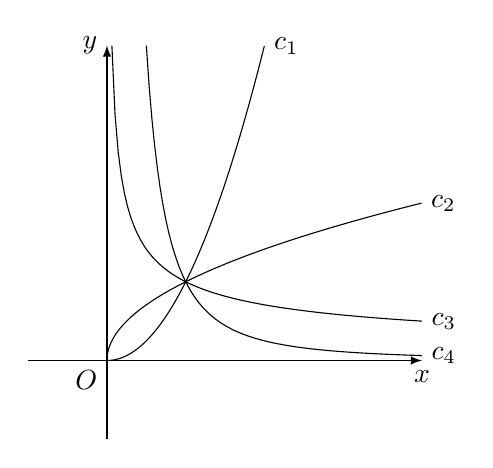
\begin{tikzpicture}[>=latex]
        \draw [->] (-1,0) -- (4,0) node [below] {$x$};
        \draw [->] (0,-1) -- (0,4) node [left] {$y$};
        \draw (0,0) node [below left] {$O$};
        \draw [domain = 0:2, samples = 100] plot (\x,\x*\x) node [right] {$c_1$};
        \draw [domain = 0:2, samples = 100] plot (\x*\x,\x) node [right] {$c_2$};
        \draw [domain = 0.0625:4, samples = 100] plot (\x, {1/sqrt(\x)}) node [right] {$c_3$};
        \draw [domain = 0.5:4, samples = 100] plot (\x, {1/\x/\x}) node [right] {$c_4$};
    \end{tikzpicture}
    \end{center}
\fourch{$-2,-\dfrac 12,\dfrac 12,2$}{$2,\dfrac 12,-\dfrac 12,-2$
}{$-\dfrac 12,-2,2,\dfrac 12$}{$2,\dfrac 12,-2,-\dfrac 12$}


关联目标:

暂未关联目标



标签: 第二单元

答案: 暂无答案

解答或提示: 暂无解答与提示

使用记录:

暂无使用记录


出处: 2022届高三第一轮复习讲义
\item { (002925)}已知幂函数$y=x^{\frac qp}$($p\in \mathbf{N}^*,\ q\in \mathbf{N}^*$, $p,q$互质)的图像如图所示, 则\bracket{20}.
\begin{center}
    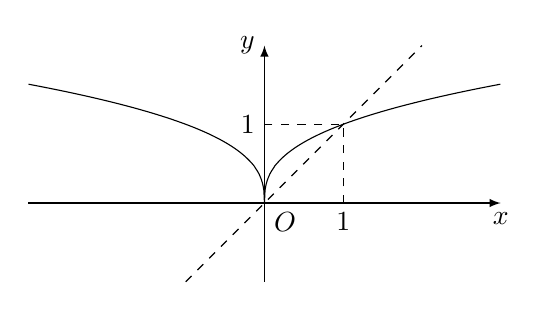
\begin{tikzpicture}[>=latex]
        \draw [->] (-3,0) -- (3,0) node [below] {$x$};
        \draw [->] (0,-1) -- (0,2) node [left] {$y$};
        \draw (0,0) node [below right] {$O$};
        \draw [dashed] (-1,-1) -- (2,2);
        \draw [domain = 0:3, samples = 400] plot (\x,{\x^(3/8)}) plot (-\x,{\x^(3/8)});
        \draw [dashed] (1,0) node [below] {$1$} -- (1,1) -- (0,1) node [left] {$1$};
    \end{tikzpicture}
\end{center}
\twoch{$p,q$均为奇数}{$p$是奇数, $q$是偶数, 且$0<\dfrac qp<1$}{$p$是偶数, $q$是奇数}{$p$是奇数, $q$是偶数, 且$\dfrac qp>1$}


关联目标:

暂未关联目标



标签: 第二单元

答案: 暂无答案

解答或提示: 暂无解答与提示

使用记录:

暂无使用记录


出处: 2022届高三第一轮复习讲义
\item { (000069)}填空题:\\
(1) 已知$m\in \mathbf{Z}$, 设幂函数$y=x^{m^2-4m}$的图像关于原点成中心对称, 且与$x$轴及$y$轴均无交点, 则$m$的值为\blank{50}.\\
(2) 设$a$、$b$为常数, 若$0<a<1$, $b<-1$, 则函数$y=a^x+b$的图像必定不经过第\blank{50}象限.


关联目标:

K0207004B|D02002B|会用图像上任意一点关于原点(或关于$y$轴)的对称点仍落在图像上证明函数的图像关于原点(或$y$轴)对称.

K0210002B|D02002B|知道指数函数图像过定点$(0,1)$.



标签: 第二单元

答案: 暂无答案

解答或提示: 暂无解答与提示

使用记录:

暂无使用记录


出处: 教材复习题
\item { (002911)}已知$\alpha\in \{-2,-1,-\dfrac 12,\dfrac 12,1,2,3\}$, 若幂函数$f(x)=x^\alpha$为奇函数, 且在$(0,+\infty)$上递减, 则$\alpha=$\blank{50}.


关联目标:

暂未关联目标



标签: 第二单元

答案: 暂无答案

解答或提示: 暂无解答与提示

使用记录:

暂无使用记录


出处: 2022届高三第一轮复习讲义
\item { (002918)}设常数$t\in \mathbf{Z}$. 已知幂函数$y=(t^3-t+1){x^{\frac 13(1+2t-t^2)}}$是偶函数, 且在区间$(0,+\infty)$上是增函数, 求整数$t$的值, 并作出相应的幂函数的大致图像.


关联目标:

暂未关联目标



标签: 第二单元

答案: 暂无答案

解答或提示: 暂无解答与提示

使用记录:

暂无使用记录


出处: 2022届高三第一轮复习讲义
\item { (005463)}幂函数$y=x^p$与$y=x^q$的图像都通过定点\blank{50}, 它们在第一象限部分关于直线$y=x$对称, 则$p,q$应满足的条件是\blank{50}.


关联目标:

暂未关联目标



标签: 第二单元

答案: 暂无答案

解答或提示: 暂无解答与提示

使用记录:

暂无使用记录


出处: 代数精编第三章函数
\item { (010137)}下列命题中, 正确的是\bracket{20}.
\onech{当$n=0$时, 函数$y=x^n$的图像是一条直线}{幂函数$y=x^n$的图像都经过$(0, 0)$和$(1, 1)$两个点}{若幂函数$y=x^n$的图像关于原点成中心对称, 则$y=x^n$在区间$(-\infty, 0)$上是严格增函数}{幂函数的图像不可能在第四象限}


关联目标:

暂未关联目标



标签: 第二单元

答案: 暂无答案

解答或提示: 暂无解答与提示

使用记录:

暂无使用记录


出处: 新教材必修第一册习题
\item { (002914)}设常数$m\in \mathbf{R}$. 若幂函数$y=(m^2-m-1)x^{m^2-2m-1}$在$(0,+\infty)$上是增函数, 则$m$的值为\blank{50}.


关联目标:

暂未关联目标



标签: 第二单元

答案: 暂无答案

解答或提示: 暂无解答与提示

使用记录:

暂无使用记录


出处: 2022届高三第一轮复习讲义
\item { (005464)}若实数$a$满足$2.4^a>2.5^a$, 求$a$的取值范围.


关联目标:

暂未关联目标



标签: 第二单元

答案: 暂无答案

解答或提示: 暂无解答与提示

使用记录:

暂无使用记录


出处: 代数精编第三章函数
\item { (005568)}若$a>b$且$ab\ne 0$.则在\textcircled{1} $a^2>b^2$, \textcircled{2} $2^a>2^b$, \textcircled{3} $\dfrac 1a<\dfrac 1b$, \textcircled{4} $a^{\frac 13}>b^{\frac 13}$, \textcircled{5} $(\dfrac 13)^a<(\dfrac 13)^b$这五个关系式中, 恒成立的有\bracket{20}.
\fourch{$1$个}{$2$个}{$3$个}{$4$个}


关联目标:

暂未关联目标



标签: 第二单元

答案: 暂无答案

解答或提示: 暂无解答与提示

使用记录:

暂无使用记录


出处: 代数精编第三章函数
\item { (009488)}(1) 已知函数$y=x^{\frac 23}$和$y=(x-1)^{\frac 23}$, 说明这两个函数图像之间的关系, 并在同一平面直角坐标系中作出它们的大致图像;\\
(2) 已知函数$y=x^{\frac 23}$和$y=x^{\frac 23}+1$, 说明这两个函数图像之间的关系, 并在同一平面直角坐标系中作出它们的大致图像.


关联目标:

暂未关联目标



标签: 第二单元

答案: 暂无答案

解答或提示: 暂无解答与提示

使用记录:

暂无使用记录


出处: 新教材必修第一册课堂练习
\item { (009490)}作出函数$y=\dfrac{-x-1}{x+2}$的大致图像.


关联目标:

暂未关联目标



标签: 第二单元

答案: 暂无答案

解答或提示: 暂无解答与提示

使用记录:

暂无使用记录


出处: 新教材必修第一册课堂练习
\item { (003815)}在同一坐标系中画出函数$y=\log_a x, \ y=a^x, y=x+a$的图像, 可能正确的是\blank{30}.
\fourch{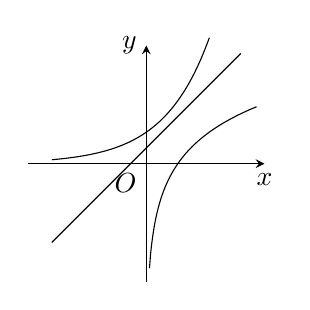
\begin{tikzpicture}[>=stealth,samples=100]
	\draw [->] (-1.5,0)--(0,0) node [below left] {$O$}--(1.5,0) node [below] {$x$};
	\draw [->] (0,-1.5)--(0,1.5) node [left] {$y$};
	\draw [domain=-3:3] plot ({\x*0.4},{(\x+0.5)*0.4});
	\draw [domain=-3:2] plot ({\x*0.4},{exp(\x*ln(2))*0.4});
	\draw [domain=0.1:3.5] plot ({\x*0.4},{ln(\x)/ln(2)*0.4});
	\end{tikzpicture}}{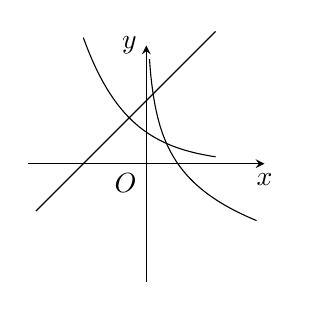
\begin{tikzpicture}[>=stealth,samples=100]
	\draw [->] (-1.5,0)--(0,0) node [below left] {$O$}--(1.5,0) node [below] {$x$};
	\draw [->] (0,-1.5)--(0,1.5) node [left] {$y$};
	\draw [domain=-3.5:2.2] plot ({\x*0.4},{(\x+2)*0.4});
	\draw [domain=-2:2.2] plot ({\x*0.4},{exp(\x*ln(1/2))*0.4});
	\draw [domain=0.1:3.5] plot ({\x*0.4},{-ln(\x)/ln(2)*0.4});
	\end{tikzpicture}}{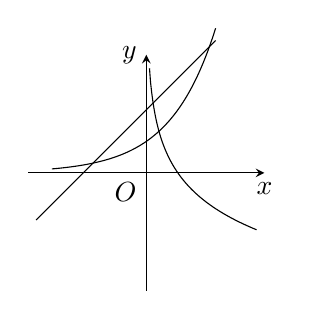
\begin{tikzpicture}[>=stealth,samples=100]
	\draw [->] (-1.5,0)--(0,0) node [below left] {$O$}--(1.5,0) node [below] {$x$};
	\draw [->] (0,-1.5)--(0,1.5) node [left] {$y$};
	\draw [domain=-3.5:2.2] plot ({\x*0.4},{(\x+2)*0.4});
	\draw [domain=-3:2.2] plot ({\x*0.4},{exp(\x*ln(2))*0.4});
	\draw [domain=0.1:3.5] plot ({\x*0.4},{-ln(\x)/ln(2)*0.4});
	\end{tikzpicture}}{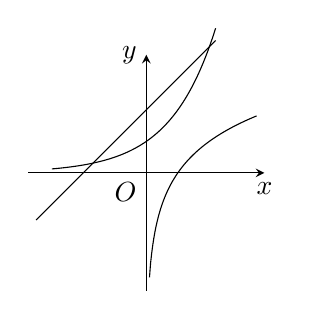
\begin{tikzpicture}[>=stealth,samples=100]
	\draw [->] (-1.5,0)--(0,0) node [below left] {$O$}--(1.5,0) node [below] {$x$};
	\draw [->] (0,-1.5)--(0,1.5) node [left] {$y$};
	\draw [domain=-3.5:2.2] plot ({\x*0.4},{(\x+2)*0.4});
	\draw [domain=-3:2.2] plot ({\x*0.4},{exp(\x*ln(2))*0.4});
	\draw [domain=0.1:3.5] plot ({\x*0.4},{ln(\x)/ln(2)*0.4});
	\end{tikzpicture}}


关联目标:

暂未关联目标



标签: 第二单元

答案: 暂无答案

解答或提示: 暂无解答与提示

使用记录:

暂无使用记录


出处: 2016年双基百分百
\item { (005569)}在同一平面直角坐标系中, 函数$f(x)=ax$与$g(x)=a^x$的图像可能是\bracket{20}.
\fourch{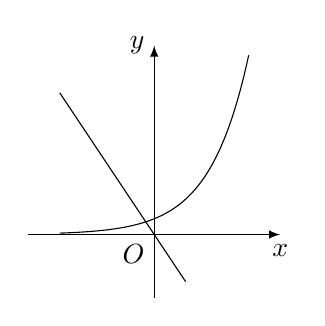
\begin{tikzpicture}[scale = 0.2, >=latex]
    \draw [->] (-8,0) -- (8,0) node [below] {$x$};
    \draw [->] (0,-4) -- (0,12) node [left] {$y$};
    \draw (0,0) node [below left] {$O$};
    \draw [domain = -6:2, samples = 100] plot (\x,{-1.5*\x});
    \draw [domain = -6:6, samples = 100] plot (\x,{1.5^\x});
\end{tikzpicture}}{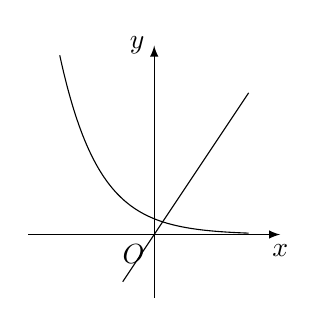
\begin{tikzpicture}[scale = 0.2, >=latex]
    \draw [->] (-8,0) -- (8,0) node [below] {$x$};
    \draw [->] (0,-4) -- (0,12) node [left] {$y$};
    \draw (0,0) node [below left] {$O$};
    \draw [domain = -2:6, samples = 100] plot (\x,{1.5*\x});
    \draw [domain = -6:6, samples = 100] plot (-\x,{1.5^\x});
\end{tikzpicture}}{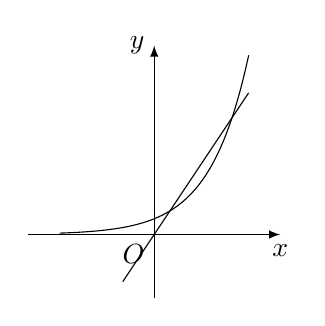
\begin{tikzpicture}[scale = 0.2, >=latex]
    \draw [->] (-8,0) -- (8,0) node [below] {$x$};
    \draw [->] (0,-4) -- (0,12) node [left] {$y$};
    \draw (0,0) node [below left] {$O$};
    \draw [domain = -2:6, samples = 100] plot (\x,{1.5*\x});
    \draw [domain = -6:6, samples = 100] plot (\x,{1.5^\x});
\end{tikzpicture}}{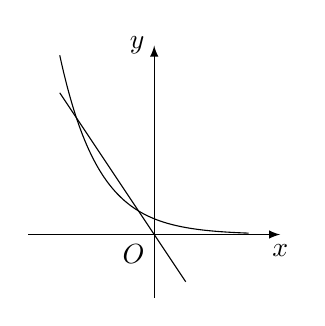
\begin{tikzpicture}[scale = 0.2, >=latex]
    \draw [->] (-8,0) -- (8,0) node [below] {$x$};
    \draw [->] (0,-4) -- (0,12) node [left] {$y$};
    \draw (0,0) node [below left] {$O$};
    \draw [domain = -2:6, samples = 100] plot (-\x,{1.5*\x});
    \draw [domain = -6:6, samples = 100] plot (-\x,{1.5^\x});
\end{tikzpicture}}


关联目标:

暂未关联目标



标签: 第二单元

答案: 暂无答案

解答或提示: 暂无解答与提示

使用记录:

暂无使用记录


出处: 代数精编第三章函数
\item { (005592)}若$0.9<a<1$, 则$a$, $a^a$, $a^{a^a}$从小到大的排列顺序是\blank{50}.


关联目标:

暂未关联目标



标签: 第二单元

答案: 暂无答案

解答或提示: 暂无解答与提示

使用记录:

暂无使用记录


出处: 代数精编第三章函数
\item { (000062)}选择题:\\
(1) 若指数函数$y=a^x$($a>0$且$a\ne 1$)在$\mathbf{R}$上是严格减函数, 则下列不等式中, 一定能成立的是\bracket{20}.
\fourch{$a>1$}{$a<0$}{$a(a-1)<0$}{$a(a-1)>0$}
(2) 在同一平面直角坐标系中, 一次函数$y=x+a$与对数函数$y=\log_ax$($a>0$且$a\ne 1$)的图像关系可能是\bracket{20}.
\fourch{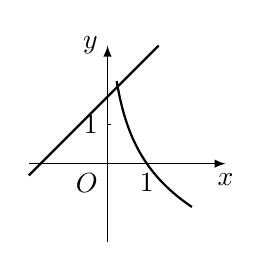
\begin{tikzpicture}[scale = 0.5,>=latex]
    \draw [->] (-2,0) -- (3,0) node [below] {$x$};
    \draw [->] (0,-2) -- (0,3) node [left] {$y$};
    \draw (0,0) node [below left] {$O$};
    \draw (0.1,1) -- (0,1) node [left] {$1$};
    \draw (1,0) node [below] {$1$};
    \draw [thick] (-2,-0.3) -- (1.3,3);
    \draw [thick,domain =-1.1:2.1,samples = 200] plot ({0.5^\x},\x);
\end{tikzpicture}
}{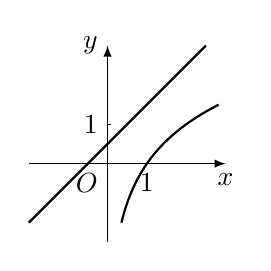
\begin{tikzpicture}[scale = 0.5,>=latex]
    \draw [->] (-2,0) -- (3,0) node [below] {$x$};
    \draw [->] (0,-2) -- (0,3) node [left] {$y$};
    \draw (0,0) node [below left] {$O$};
    \draw (0.1,1) -- (0,1) node [left] {$1$};
    \draw (1,0) node [below] {$1$};
    \draw [thick] (-2,-1.5) -- (2.5,3);
    \draw [thick,domain =1.5:-1.5,samples = 200] plot ({0.5^\x},-\x);
\end{tikzpicture}
}{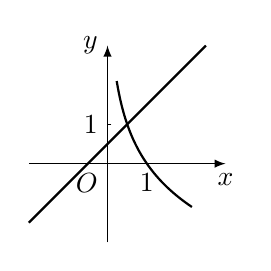
\begin{tikzpicture}[scale = 0.5,>=latex]
    \draw [->] (-2,0) -- (3,0) node [below] {$x$};
    \draw [->] (0,-2) -- (0,3) node [left] {$y$};
    \draw (0,0) node [below left] {$O$};
    \draw (0.1,1) -- (0,1) node [left] {$1$};
    \draw (1,0) node [below] {$1$};
    \draw [thick] (-2,-1.5) -- (2.5,3);
    \draw [thick,domain =-1.1:2.1,samples = 200] plot ({0.5^\x},\x);
\end{tikzpicture}
}{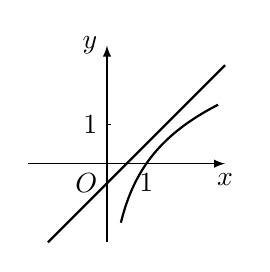
\begin{tikzpicture}[scale = 0.5,>=latex]
    \draw [->] (-2,0) -- (3,0) node [below] {$x$};
    \draw [->] (0,-2) -- (0,3) node [left] {$y$};
    \draw (0,0) node [below left] {$O$};
    \draw (0.1,1) -- (0,1) node [left] {$1$};
    \draw (1,0) node [below] {$1$};
    \draw [thick] (-1.5,-2) -- (3,2.5);
    \draw [thick,domain =1.5:-1.5,samples = 200] plot ({0.5^\x},-\x);
\end{tikzpicture}
}


关联目标:

K0211001B|D02002B|会利用指数函数的单调性解决相关不等式等问题.

K0213007B|D02002B|会作出对数函数的大致图像, 能根据其图像特征叙述函数性质.



标签: 第二单元

答案: 暂无答案

解答或提示: 暂无解答与提示

使用记录:

暂无使用记录


出处: 教材复习题
\item { (000738)}函数$f(x)=\lg (3^x-2^x)$的定义域为\blank{50}.


关联目标:

暂未关联目标



标签: 第二单元

答案: $(0,+\infty)$

解答或提示: 暂无解答与提示

使用记录:

20220427	2022届高三1班	\fcolorbox[rgb]{0,0,0}{1.000,0.280,0}{0.860}


出处: 赋能练习
\item { (000954)}函数$y=\sqrt{2^x-1}$的定义域是\blank{50}(用区间表示).


关联目标:

暂未关联目标



标签: 第二单元

答案: $[0,+\infty)$

解答或提示: 暂无解答与提示

使用记录:

20220628	2022届高三1班	\fcolorbox[rgb]{0,0,0}{1.000,0.000,0}{1.000}


出处: 赋能练习
\item { (001345)}解方程: $3^x+4^x=5^x$.


关联目标:

暂未关联目标



标签: 第二单元

答案: 暂无答案

解答或提示: 暂无解答与提示

使用记录:

2016届11班	\fcolorbox[rgb]{0,0,0}{1.000,0.206,0}{0.897}

2016届12班	\fcolorbox[rgb]{0,0,0}{1.000,0.054,0}{0.973}


出处: 2016届创新班作业	1157-指数方程
\item { (001343)}方程$9^x+4^x=\dfrac{5}{2}\cdot 6^x$的解集为\blank{80}.


关联目标:

暂未关联目标



标签: 第二单元

答案: 暂无答案

解答或提示: 暂无解答与提示

使用记录:

2016届11班	\fcolorbox[rgb]{0,0,0}{1.000,0.410,0}{0.795}

2016届12班	\fcolorbox[rgb]{0,0,0}{1.000,0.432,0}{0.784}


出处: 2016届创新班作业	1157-指数方程
\item { (001324)}函数$y=\log_{x^2+x-1} 2$的定义域是\blank{150}.


关联目标:

暂未关联目标



标签: 第二单元

答案: 暂无答案

解答或提示: 暂无解答与提示

使用记录:

2016届11班	\fcolorbox[rgb]{0,0,0}{1.000,0.158,0}{0.921}

2016届12班	\fcolorbox[rgb]{0,0,0}{1.000,0.052,0}{0.974}


出处: 2016届创新班作业	1155-对数函数
\item { (001326)}函数$y=\log_2(x^2+x-1)$的定义域是\blank{80}, 值域是\blank{80}.


关联目标:

暂未关联目标



标签: 第二单元

答案: 暂无答案

解答或提示: 暂无解答与提示

使用记录:

2016届11班	\fcolorbox[rgb]{0,0,0}{1.000,0.106,0}{0.947}

2016届12班	\fcolorbox[rgb]{0,0,0}{1.000,0.106,0}{0.947}


出处: 2016届创新班作业	1155-对数函数
\item { (001329)}已知函数$f(x)=\lg(kx^2-6x+k+3)$的定义域为$\mathbf{R}$, 则$k$的取值范围为\blank{80}.


关联目标:

暂未关联目标



标签: 第二单元

答案: 暂无答案

解答或提示: 暂无解答与提示

使用记录:

2016届11班	\fcolorbox[rgb]{0,0,0}{1.000,0.316,0}{0.842}

2016届12班	\fcolorbox[rgb]{0,0,0}{1.000,0.422,0}{0.789}


出处: 2016届创新班作业	1155-对数函数
\item { (002871)}设常数$a\in \mathbf{R}$.若直线$x=2$是函数$f(x)=\log_3|2x+a|$的图像的一条对称轴, 则$a$=\blank{50}.


关联目标:

暂未关联目标



标签: 第二单元

答案: 暂无答案

解答或提示: 暂无解答与提示

使用记录:

暂无使用记录


出处: 2022届高三第一轮复习讲义
\item { (003041)}已知实数$ab$满足等式$(\dfrac 12)^a=(\dfrac 13)^b$, 下列五个关系式:\\
\textcircled{1} $0<b<a$; \textcircled{2} $a<b<0$; \textcircled{3} $0<a<b$; \textcircled{4} $b<a<0$; \textcircled{5} $a=b=0$. 其中不可能成立的关系式的序号为\blank{50}.


关联目标:

暂未关联目标



标签: 第二单元

答案: 暂无答案

解答或提示: 暂无解答与提示

使用记录:

暂无使用记录


出处: 2022届高三第一轮复习讲义
\item { (002874)}函数$y=\log_2\dfrac{2-x}{2+x}$的图像关于\bracket{20}.
\fourch{原点对称}{$y$轴对称}{直线$y=x$对称}{直线$y=-x$对称}


关联目标:

暂未关联目标



标签: 第二单元

答案: 暂无答案

解答或提示: 暂无解答与提示

使用记录:

暂无使用记录


出处: 2022届高三第一轮复习讲义
\item { (002875)}函数$y=\log_2(2-2^x)$的图像关于\bracket{20}.
\fourch{原点对称}{$y$轴对称}{直线$y=x$对称}{直线$y=-x$对称}


关联目标:

暂未关联目标



标签: 第二单元

答案: 暂无答案

解答或提示: 暂无解答与提示

使用记录:

暂无使用记录


出处: 2022届高三第一轮复习讲义
\item { (002878)}设函数$y=\log_2(x+3)$的图像与函数$y=f(x)$的图像关于直线$x=1$对称. \textcircled{1} $f(1)$=\blank{50}; \textcircled{2} 若$f(a)$有意义, 则$f(a)=$\blank{50}(结果用$a$的表达式表示).


关联目标:

暂未关联目标



标签: 第二单元

答案: 暂无答案

解答或提示: 暂无解答与提示

使用记录:

暂无使用记录


出处: 2022届高三第一轮复习讲义
\item { (005720)}若函数$f(x)=|\log_ax|$, 其中$0<a<1$, 则下列各式中成立的是\bracket{20}.
\fourch{$f(\dfrac 13)>f(2)>f(\dfrac 14)$}{$f(\dfrac 14)>f(\dfrac 13)>f(2)$}{$f(2)>f(\dfrac 13)>f(\dfrac 14)$}{$f(\dfrac 14)>f(2)>f(\dfrac 13)$}


关联目标:

暂未关联目标



标签: 第二单元

答案: 暂无答案

解答或提示: 暂无解答与提示

使用记录:

暂无使用记录


出处: 代数精编第三章函数
\item { (001325)}函数$y=\log_2(x^2+x-1)$的递增区间是\blank{150}.


关联目标:

暂未关联目标



标签: 第二单元

答案: 暂无答案

解答或提示: 暂无解答与提示

使用记录:

2016届11班	\fcolorbox[rgb]{0,0,0}{1.000,0.894,0}{0.553}

2016届12班	\fcolorbox[rgb]{0,0,0}{1.000,0.736,0}{0.632}


出处: 2016届创新班作业	1155-对数函数
\item { (002898)}函数$y=\log_{0.7}(x^2-3x+2)$的单调减区间为\blank{50}.


关联目标:

暂未关联目标



标签: 第二单元

答案: 暂无答案

解答或提示: 暂无解答与提示

使用记录:

暂无使用记录


出处: 2022届高三第一轮复习讲义
\item { (002905)}设常数$a\in \mathbf{R}$.若函数$f(x)=\log_a(2-ax)$在$[0,1]$上是减函数, 求$a$的取值范围.


关联目标:

暂未关联目标



标签: 第二单元

答案: 暂无答案

解答或提示: 暂无解答与提示

使用记录:

暂无使用记录


出处: 2022届高三第一轮复习讲义
\item { (000063)}求下列函数的的定义域:\\
(1) $y=(x-1)^{\frac 52}$;\\
(2) $y=3^{\sqrt{x-1}}$;\\
(3) $y=\lg \dfrac{1+x}{1-x}$.


关联目标:

K0207002B|D02002B|会根据具体的幂指数$a$求解幂函数$y=x^{a}$的定义域.

K0209002B|D02002B|会求解有关指数型函数的定义域.

K0212002B|D02002B|会求解有关对数型函数的定义域.



标签: 第二单元

答案: 暂无答案

解答或提示: 暂无解答与提示

使用记录:

暂无使用记录


出处: 教材复习题
\item { (001330)}已知函数$f(x)=\lg(kx^2-6x+k+3)$的值域为$\mathbf{R}$, 则$k$的取值范围为\blank{80}.


关联目标:

暂未关联目标



标签: 第二单元

答案: 暂无答案

解答或提示: 暂无解答与提示

使用记录:

2016届11班	\fcolorbox[rgb]{0,0,0}{1.000,1.000,0}{0.500}

2016届12班	\fcolorbox[rgb]{0,0,0}{0.790,1.000,0}{0.395}


出处: 2016届创新班作业	1155-对数函数
\item { (000362)}方程$\log_2(9^x-5)=2+\log_2(3^x-2)$的解$x=$\blank{50}.


关联目标:

暂未关联目标



标签: 第二单元

答案: $x=1$

解答或提示: 暂无解答与提示

使用记录:

20211210	2022届高三1班	\fcolorbox[rgb]{0,0,0}{1.000,0.136,0}{0.932}


出处: 赋能练习
\item { (004902)}若$a=\log_{0.2}0.3$, $b=\log_{0.3}0.2$, $c=1$, 则$a,b,c$的大小关系是\bracket{20}.
\fourch{$a>b>c$}{$b>a>c$}{$b>c>a$}{$c>b>a$}


关联目标:

暂未关联目标



标签: 第一单元|第二单元

答案: 暂无答案

解答或提示: 暂无解答与提示

使用记录:

暂无使用记录


出处: 代数精编第二章不等式
\item { (004907)}若$x>y>1$, $0<a<1$, 则下列各式中正确的一个是\bracket{20}.
\fourch{${x^{-a}}>{y^{-a}}$}{$(\sin a)^x>(\sin a)^y$}{$\log_{\frac 1a}x<\log_{\frac 1a}y$}{$1+a^{x+y}>a^x+a^y$}


关联目标:

暂未关联目标



标签: 第一单元|第二单元|第三单元

答案: 暂无答案

解答或提示: 暂无解答与提示

使用记录:

暂无使用记录


出处: 代数精编第二章不等式
\item { (000075)}仅利用对数函数的单调性和计算器上的乘方功能来确定对数$\log_23$第二位小数的值.


关联目标:

K0214001B|D02002B|会利用对数函数的单调性估算对数型无理数(如$\log_23$).



标签: 第二单元

答案: 暂无答案

解答或提示: 暂无解答与提示

使用记录:

暂无使用记录


出处: 教材复习题
\item { (000567)}函数$f(x)=\sqrt{1-\lg x}$的定义域为\blank{50}.


关联目标:

暂未关联目标



标签: 第二单元

答案: $(0,10 ]$

解答或提示: 暂无解答与提示

使用记录:

20220315	2022届高三1班	\fcolorbox[rgb]{0,0,0}{1.000,0.094,0}{0.953}


出处: 赋能练习
\item { (000795)}若函数$f(x)={\log_a}(x^2-ax+1)\ (a>0, \ a\ne 1)$没有最小值, 则$a$的取值范围是\blank{50}.


关联目标:

暂未关联目标



标签: 第二单元

答案: $(0,1)\cup [2,+\infty)$

解答或提示: 暂无解答与提示

使用记录:

20220511	2022届高三1班	\fcolorbox[rgb]{0,0,0}{1.000,0.512,0}{0.744}

20220622	2022届高三1班  	\fcolorbox[rgb]{0,0,0}{1.000,0.232,0}{0.884}


出处: 赋能练习
\item { (001328)}不等式$\log_{\frac{1}{2}}(x^2+x+1)<\log_{\frac{1}{2}}(4x-1)$的解集为\blank{80}.


关联目标:

暂未关联目标



标签: 第二单元

答案: 暂无答案

解答或提示: 暂无解答与提示

使用记录:

2016届11班	\fcolorbox[rgb]{0,0,0}{1.000,0.684,0}{0.658}

2016届12班	\fcolorbox[rgb]{0,0,0}{1.000,1.000,0}{0.500}


出处: 2016届创新班作业	1155-对数函数
\item { (001351)}若函数$f(x)=\log_a x$在区间$[a,2a]$上的最大值与最小值之差为$\dfrac{1}{2}$, 则$a=$\blank{100}.


关联目标:

暂未关联目标



标签: 第二单元

答案: 暂无答案

解答或提示: 暂无解答与提示

使用记录:

2016届11班	\fcolorbox[rgb]{0,0,0}{1.000,0.154,0}{0.923}

2016届12班	\fcolorbox[rgb]{0,0,0}{1.000,0.162,0}{0.919}


出处: 2016届创新班作业	1158-对数方程
\item { (001352)}解方程: $\log_x(x^2-x)\le \log_x 2$.


关联目标:

暂未关联目标



标签: 第二单元

答案: 暂无答案

解答或提示: 暂无解答与提示

使用记录:

2016届11班	\fcolorbox[rgb]{0,0,0}{1.000,0.206,0}{0.897}

2016届12班	\fcolorbox[rgb]{0,0,0}{1.000,0.270,0}{0.865}


出处: 2016届创新班作业	1158-对数方程
\item { (003747)}若$\log_a \dfrac 23<1 \ (a>0, \ a\ne 1)$, 则实数$a$的取值范围为\blank{50}.


关联目标:

暂未关联目标



标签: 第二单元

答案: 暂无答案

解答或提示: 暂无解答与提示

使用记录:

暂无使用记录


出处: 2016年双基百分百
\item { (005199)}解关于$x$的不等式: $\log_{\frac 12}(3x-2)>\log_{\frac 12}(x+1)$.


关联目标:

暂未关联目标



标签: 第二单元

答案: 暂无答案

解答或提示: 暂无解答与提示

使用记录:

暂无使用记录


出处: 代数精编第二章不等式
\item { (005723)}若$a>a^2>b>0$, 并记$p=\log_ab$, $q=\log_ba$, $r=\log_a\dfrac ab$, $s=\log_b\dfrac ba$, 则$p,q,r,s$的大小关系是\bracket{20}.
\fourch{$r<q<p<s$}{$r<p<q<s$}{$r<p<s<q$}{$r<q<s<p$}


关联目标:

暂未关联目标



标签: 第二单元

答案: 暂无答案

解答或提示: 暂无解答与提示

使用记录:

暂无使用记录


出处: 代数精编第三章函数
\item { (005724)}若$\log_a\dfrac 13>\log_b\dfrac 13>0$, 则$a,b$的关系是\bracket{20}.
\fourch{$1<b<a$}{$1<a<b$}{$0<a<b<1$}{$0<b<a<1$}


关联目标:

暂未关联目标



标签: 第二单元

答案: 暂无答案

解答或提示: 暂无解答与提示

使用记录:

暂无使用记录


出处: 代数精编第三章函数
\item { (010162)}若$a>b>c>1$, 则下列不等式不成立的是\blank{50}. (填写所有不成立的不等式的序号)\\
\textcircled{1} $\log_ab>\log_ac$; \textcircled{2} $\log_a\dfrac 1b>\log_a\dfrac 1c$; \textcircled{3} $\log_{\frac 1a}b>\log_{\frac 1a}c$; \textcircled{4} $\log_{\frac 1a}\dfrac 1b>\log_{\frac 1a}\dfrac 1c$.


关联目标:

暂未关联目标



标签: 第二单元

答案: 暂无答案

解答或提示: 暂无解答与提示

使用记录:

暂无使用记录


出处: 新教材必修第一册习题
\end{enumerate}



\end{document}